\clearpage

\subsection{Olika trafiksätt på HF}

De olika HF-banden har olika egenskaper över tid på dagen, tid på året och påverkas vädligt mycket av rådande rymdväder och hur joniserat den övre delen av atmosfären är för att bilda rymdvåg.

Med det stora antalet band som radioamatörer förfogar över så finns det ofta något band som fungerar. Det gäller att man lär sig hur de olika egenskaperna påverkar de olika banden och när man kan förvänta sig att de ''öppnar'' och fungerar på längre avstånd.

Klassiska amatörradioband på kortvågen är därför 160 meter (som ju egentligen är ett gränsvågsband då det ligger precis under kortvågen enligt rådande ITU-definition), 80, 40, 60, 20, 17, 15, 12 och 10 metersbanden ger radioamatörer en stor karta av olika band att arbeta med.

För den som inte är radioamatör så är urvalet mer begränsat och även den effekt man lagligen får använda. Här finns egentligen bara 27~MHz och till nöds kan man väl även räkna jaktfrekvenserna på 31~MHz också men begränsningen i användandet och vilken effekt som står till buds gör att kortvågen är radioamatörernas jaktmark i första hand.

Vi ska i det här kapitlet titta lite på de olika bandens olika egenskaper och lite olika sätt att använda dem för att nå lokalt, lite längre och DX -- dvs i det närmaste globalt.

\subsubsection{Solens inverkan -- rymdvädret}

En sak som har mycket kraftig inverkan på radiosamband på kortvåg är rymdvädret. Som många känner till så följer solens solfläckar en 11-årig cykel och just nu inväntar vi toppen på cykel nummer 25 (numrerad från 1 sedan man började numrera dem) och dess topp förväntas inträffa under 2025. Därefter kommer vi se en nedgång i solfläckar fram till början av nästa cykel, som då blir cykel 26. 

I botten på solfläckscyklerna blir det ofta sämre så kallade konditioner på kortvågsbanden. Det blir svårare att nå långt och hitta ''öppningar'' på banden med högre frekvens, framför allt 15-, 12- och 10-metersbanden. Lokalt fungerar de bra men för de där riktiga DX-öppningarna behövs lite solaktivitet.

I toppen på solcykeln kan det däremot vara väldigt varierande. Ena dagen har man enorma öppningar på 10-metersbandet så att man kan kommunicera lokalt, men risken för en kraftig så kallad ''flare'' från solen eller en CME (koronal mass-utkasning, Coronal Mass Ejection) där en del av solens yta slungas iväg i kraftiga explosioner påverkar inte bara solvindens möjligheter att jonisera de övre luftlagren utan kan också skapa störningar i det jordmagnetiska fältet.

När detta sker brukar det åtföljas av kraftiga och vackra polarsken (norrksen i norr och sydsken i syd) och amatörerna benämner dessa som ''aurora''. Då denna uppträder är ofta kortvågen kraftigt påverkad på ett negativt sätt men ibland kan man nyttja själva auroran och studsa lite högre frekvenser på den som t.ex. VHF och då exempelvis 6-metersbandet eller 2-metersbandet.

\subsubsection{Markvåg}

Precis som för VHF och UHF så finns det på kortvåg också en markvåg. Den är dock relativt begränsad i sin utbredning och kommer något längre än den sträcka man kan beräkna med formler för VHF, dvs radiohorisonten. Kortvåg har en förmåga att ta sig en smula längre i alla fall men främst är det rymdvågsegenskaperna som är den intressanta.

\subsubsection{Rymdvåg}

Rymdvågen är den utbrednignsform som gör kortvåg till ett globalt kommunikationsmedel. Genom att den övre delen av atmosfären joinseras av solens strålning -- jonosfären -- så kommer också radiovågor under en viss frekvens att kunna studsa mot dessa.

Denna frekvens kallas för MUF (maximum useable frequency) och betyder i praktiken den högsta frekvensen som fortfarande reflekteras i jonosfären. Frekvenser under MUF går också att använda men frekvenser över MUF fungerar mycket dåligt.

På olika ställen runt jorden mäts MUF genom så kallade ''jonosonder'' som innebär att man skickar en svept signal, ofta från ca 2~MHz till ungefär 40~MHz och sedan lyssnar man på olika mottagarstationer vad som kommer tillbaka och hur starkt det är. På amatörradions mottagare kan man ibland höra ett sådant svep och då är det reflexten av jonosonden som man hör.

\subsubsection{Generellt om kortvågbandens rymdvåg}

Lägre frekvenser reflekteras oftast på lägre nivå i jonosfären, de tränger inte lika högt upp i de olika reflekterande lagren innan de reflekteras. På samma sätt reflekteras i regel högre frekvenser högre upp. Detta gör att givet en viss vinkel så kommer den reflekterade rymdvågen ner på olika ställen, olika långt bort från sändaren, beroende på frekvensen. 

För att komma så långt som möjligt bör man välja ett band som är så nära MUF som möjligt och ha en relativt flack vinkel från sin antenn. För att uppnå NVIS skickar man signalen med en brant vinkel, nästan vertikalt uppåt, och den kommer då tillbaka ganska rakt uppifrån.

\subsubsection{NVIS}

Ett särskilt sätt att sända kortvåg är att skicka signalen nästan rakt uppåt. Sättet kallas på engelska för ''Near Vertical Incidence Skywave'' och kan översättas ungefär som ''nästan vertikalt vinklad rymdvåg'' och innebär att man placerar en kortvågsantenn relativt lågt, ibland bara några meter över mark. Man får då en våg som riktas i det närmaste rakt uppåt då marken agerar som en mycket nära reflektor.

Denna typ av rymdvåg träffar då de joniserade delarna av atmosfären och reflekteras tillbaka till marka, man kan beskriva det ungefär som ett ''paraply'' av signaler som kommer ner. Radien är ofta mellan 400--600~km vilket gör att man kan täcka in en stor del av skandinavien och norra Europa med NVIS.

Lämpliga band för NVIS är band mellan 2--8 MHz så för oss radioamatörer blir det då 160-, 80-, 40-metersbanden främst, men även 60-metersbandet kan nyttjas för NVIS.

%\begin{figure}[h]
%	\centering
%	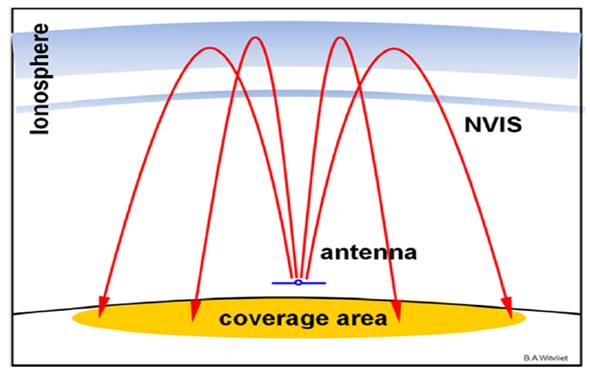
\includegraphics[width=0.6\textwidth]{bilder/NVIS-Propagation}
%	\label{fig:nvis-propagation}
%	\caption{NVIS-utbredning, princip}
%\end{figure}

NVIS används mycket på t.ex. 80-metersbandet för olika ''ringar'' och liknande när man träffas flera sändaramatörer på en viss frekvens en viss tid och sedan turas om att sända och kommentera på olika saker. 

\subsubsection{DX -- långväga kontakter}

För mer långväga kontakter lägger vi oss så högt det går, har antenner som sänder i en flackare vinkel, nästan rakt mot horisonten på lite högre höjd om möjligt och gärna också riktantenner i stället för de vanliga dipolerna som är den vanligaste antennen för de lägre kortvågsbanden.

Genom att kombinera detta och reflektera så högt upp i jonosfären som möjligt kan vi ibland nå mycket långt. Är konditionerna goda kan man få flera sådana hopp (skip) efter varandra och på så vis kan vi nå till andra sidan planeten. Vid gynnsamma konditioner kan man med relativt enkla medel prata med Japan och Australien på kortvåg.

\subsection{Bandens olika egenskaper}

\todo{Beskriva}

\subsubsection{160--80 meter}
\todo{Beskriva}


\subsubsection{40-60 meter}
\todo{Beskriva}

\subsubsection{20, 17, 12 och 10 meter}
\todo{Beskriva}

